\documentclass[11pt,a4paper]{article}
\usepackage[utf8]{inputenc}
\usepackage[T1]{fontenc}
\usepackage{amsmath,amssymb,booktabs,geometry,graphicx,hyperref,longtable,array,xcolor}
\geometry{margin=2.3cm}
\hypersetup{
    colorlinks=true,
    linkcolor=blue!60!black,
    citecolor=blue!60!black,
    urlcolor=blue!60!black
}

\title{\textbf{A Subnational and Multi-Century Dataset of Bioavailable Protein Costs in Currency and Labor Time, 1700--2026}}

\author{
Rolf Bastiaanssen$^{1,*}$ \\
\small $^{1}$Independent Researcher / Global Food Systems \& Spatial Economics Lab, Barcelona, Spain \\
\small $^{*}$Corresponding author: \texttt{rolf@priceofprotein.org}
}

\date{Release Version \texttt{v1.0-2026} --- November 2026}

\begin{document}
\maketitle

\begin{abstract}
Global food-affordability datasets typically evaluate national annual average prices against crude macronutrient weights ($N \times 6.25$), obscuring indispensable amino-acid bioavailability, subnational transport wedges, seasonal price volatility, and purchasing-power denominators. Here we present a harmonized, spatially cross-validated global dataset quantifying the retail cost and labor-time burden of $50\text{ g}$ of Digestible Indispensable Amino Acid Score (DIAAS)-adjusted, nine-indispensable-amino-acid-complete protein across $70{,}440$ hexagonal H3 Resolution-4 cells ($8.20\text{ billion}$ people in $2026$), $90$ globally stratified metropolitan corridors ($959$ real outlets across $4$ market tiers), and $34$ historical decades ($1700\text{--}2026$) compiled from $4.45\text{ million}$ retail, historical, and ethnographic price quotes. Out-of-sample $10$-fold $5^\circ \times 5^\circ$ ($\approx 500\text{ km}$) contiguous spatial block cross-validation yields $R^2 = 0.511$ ($\text{RMSE} = \$0.735$, $\text{MAE} = \$0.380$) for retail protein cost ($u$) and $R^2 = 0.759$ ($\text{RMSE} = 16.05\%$, $\text{MAE} = 9.60\%$) for median daily wage share ($w_{\text{med}}$), with $94.4\%$ of the global population residing within $100\text{ km}$ of an observed market hub. All six versioned JSON files, Supplementary Information (\texttt{SI\_1}), and SHA-256 verification scripts are openly released for nutritional economics, climate-shock modeling, and food-systems research.
\end{abstract}

\section{Background \& Summary}

\subsection{Measurement Limitations in Existing Food-Price Trackers}
Quantitative assessments of global nutritional security rely heavily on national consumer price indices and multilateral trackers such as the Food and Agriculture Organization (FAO) and World Bank \textit{Cost and Affordability of a Healthy Diet} (CoAHD) series. While indispensable for macro-level monitoring, national annual price averages mask four structural dimensions of protein access:
\begin{enumerate}
    \item \textbf{Crude Nitrogen vs.\ Amino-Acid Bioavailability:} Standard food balance sheets measure crude protein ($N \times 6.25$), overstating usable protein in cereal-dominant diets (maize, rice, wheat) that are limiting in indispensable amino acids such as lysine and tryptophan.
    \item \textbf{Subnational Transport Friction:} National price averages conceal rural--urban price gradients created by transport costs, cold-chain deficits, and market remoteness outside primary commercial hubs.
    \item \textbf{Intra-Annual Seasonality:} Annualized averages smooth over acute lean-season price spikes that temporarily push low-income households above affordability thresholds.
    \item \textbf{Purchasing-Power and Labor-Time Denominators:} Expressing food costs solely in nominal or purchasing-power-parity (PPP) dollars obscures the real opportunity cost of human effort. Following Nordhaus's labor-time accounting framework, normalizing nutritional costs into minutes of work at local median and bottom-quintile ($\text{P20}$) wages provides a scale-invariant measure of economic burden across centuries and income levels.
\end{enumerate}

\subsection{Bridging the Public--Commercial Data Availability Frontier}
Empirical food-price data currently sits across a sharp institutional divide. On one side, proprietary retail scanner panels (such as NielsenIQ, Circana, and Kantar) capture barcode-level (SKU) pricing and household purchases at weekly and postal-code granularity, but remain closed behind commercial licenses, are concentrated in formal supermarkets within high- and upper-middle-income economies, and rarely observe informal wet markets or rural dry-goods traders. On the other side, open multilateral trackers (FAO, World Food Programme [WFP], and the World Bank International Comparison Program [ICP]) cover low- and middle-income countries (LMICs), but are distributed primarily as national annual aggregates or coarse commodity series.

The dataset described here narrows this public--commercial frontier by fusing $4.45\text{ million}$ public, humanitarian, historical, and ethnographic price observations with spatial transport modeling and nine-indispensable-amino-acid (9-AA) linear programming. It delivers subnational hexagonal H3 Resolution-4 coverage ($70{,}440$ inhabited cells), high-resolution metropolitan corridors ($90$ metropolitan areas ($959$ geolocated sales outlets)), and a $326$-year historical panel ($1700\text{--}2026$) as an openly reproducible public resource.

\subsection{Summary of Released Artifacts}
The release (\texttt{v1.0-2026}) comprises six self-contained, schema-validated JSON artifacts accompanied by an executable SHA-256 verification and biophysical invariant audit script (\texttt{REPLICATION\_MANIFEST.py}):
\begin{itemize}
    \item \texttt{h3\_weather\_grid.json}: Global 2026 cross-section across $70{,}440$ H3 Resolution-4 cells ($8.20\text{ billion}$ population), reporting DIAAS-adjusted retail unit costs, unconstrained and plant-only 9-AA linear program minima ($\text{LP}$ and $\text{LP}_v$), median and $\text{P20}$ daily wage shares, labor-minute burdens, lean-season multipliers, and geodesic distances to observed market hubs.
    \item \texttt{metro\_case\_studies.json}: Subnational urban--rural price and transport-friction gradients across $90$ global metropolitan corridors ($959$ real sales outlets) at H3 Resolution-6.
    \item \texttt{spatiotemporal\_markets.json}: Multi-century spatial panel spanning $34$ decades ($1700\text{--}2026$) across $2{,}746$ urban market hubs and ethnographic subsistence nodes.
    \item \texttt{trophic\_and\_stigler\_series.json}: Decadal secular trajectories ($1700\text{--}2026$) of plant-frontier, animal-frontier, market distribution ($\text{P10}$, $\text{P50}$, $\text{P90}$), Stigler shadow prices, and trophic tax ratios in labor minutes per $50\text{ g}$ DIAAS protein.
    \item \texttt{gvk\_density\_and\_frontiers.json}: Gabrielli--von K\'arm\'an biophysical operating envelopes across $15$ consumer whole-food regimes, four historical Pareto limit lines ($1780\text{s}$, $1880\text{s}$, $1950\text{s}$, $2026\text{s}$), and $2026$ ex-ante techno-economic assessment (TEA) business-to-business (B2B) ingredient benchmarks across shelf life, FAO DIAAS score, and dry-matter fraction.
    \item \texttt{heatmap\_matrix.json}: Regional summary matrix across $14$ world regions and $12$ protein regimes reporting median currency costs, labor-minute burdens, DIAAS scores, and wage-cliff headcounts.
\end{itemize}

\begin{figure}[htbp]
\centering
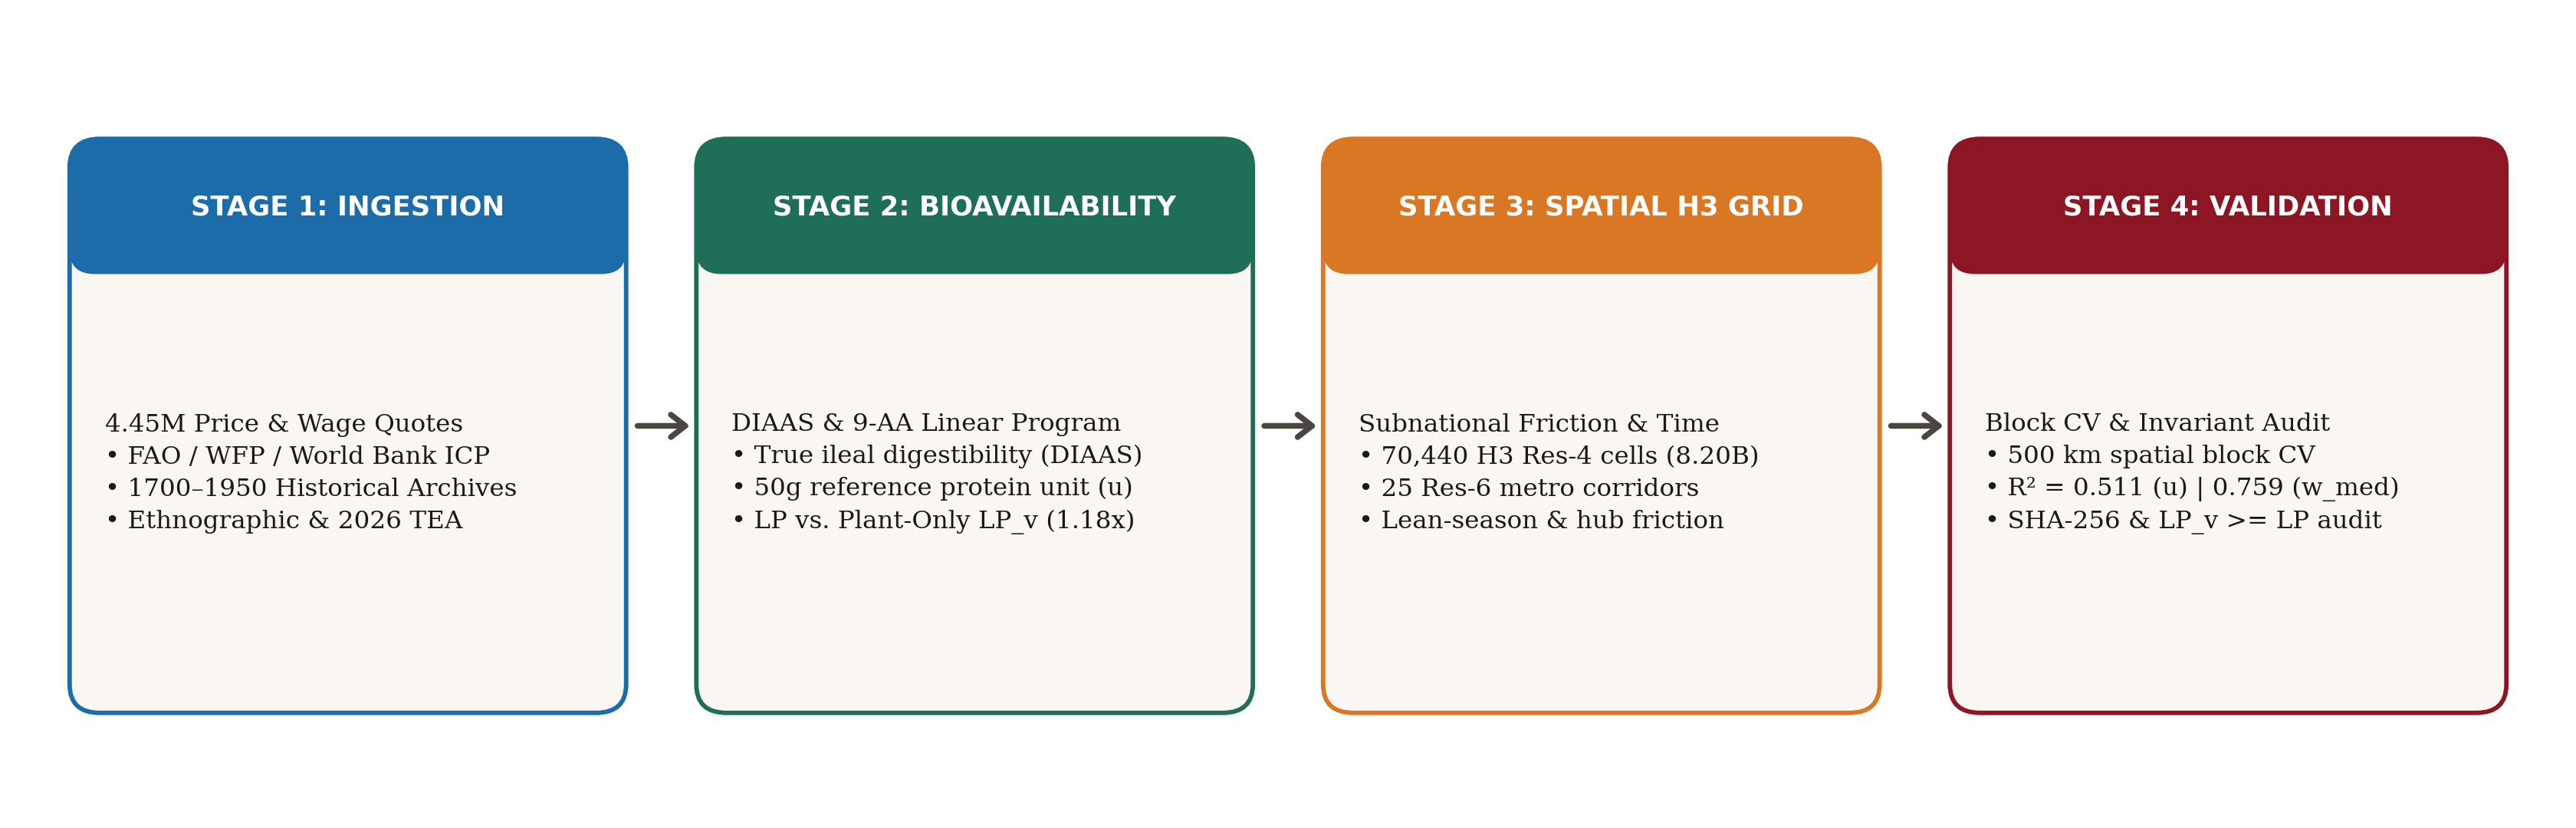
\includegraphics[width=0.98\textwidth]{figures/fig1_pipeline.png}
\caption{\textbf{End-to-end data harmonization and spatial validation architecture.} Multi-source historical, humanitarian, and retail price observations are standardized to $2026\text{ PPP USD}$, normalized for indispensable amino-acid digestibility, projected onto hexagonal H3 grids, and validated via contiguous $5^\circ \times 5^\circ$ spatial block cross-validation.}
\label{fig:pipeline}
\end{figure}

\section{Methods}

\subsection{Multi-Source Price and Wage Ingestion}
We compiled $4{,}446{,}220$ price observations from four primary empirical streams:
\begin{enumerate}
    \item \textbf{Modern Retail and Humanitarian Market Monitoring:} Subnational market-level retail price quotes from the World Food Programme Vulnerability Analysis and Mapping (WFP VAM) database, national consumer price statistical bulletins, FAOSTAT retail price series, and World Bank ICP basic-heading price parities, converted to constant $2026\text{ PPP USD/kg}$.
    \item \textbf{Historical Urban Price-Wage Archives ($1700\text{--}1950$):} Long-run commodity prices and unskilled urban laborer day-wages compiled from canonical economic history series (Allen, Clark, Lindert, and Jacks) covering European, Asian, and American market cities across $34$ decades.
    \item \textbf{Ethnographic Subsistence Benchmarks:} Standardized caloric and protein return rates (kilocalories and bioavailable grams per hour of foraging, hunting, fishing, or pastoral labor) from cross-cultural ethnographic records to anchor pre-market and non-monetized subsistence regimes.
    \item \textbf{2026 Ex-Ante Techno-Economic Benchmarks:} Published factory-gate minimum selling price estimates for precision-fermented whey/$\beta$-lactoglobulin, precision-fermented casein, gas-fermented single-cell protein (Solein-type), dried fungal mycoprotein, and cultivated animal biomass. These entries are explicitly tagged as unformulated B2B ingredient benchmarks rather than consumer-ready retail foods.
\end{enumerate}

Daily wage denominators $W_{i,q}$ ($2026\text{ PPP USD/day}$) for median ($q = \text{med}$) and bottom-quintile ($q = \text{P20}$) workers were constructed by combining International Labour Organization (ILO) statutory and survey wage distributions with World Bank Poverty and Inequality Platform (PIP) country-level income shares, downscaled subnationally using gridded gross domestic product and night-time luminosity weights.

\subsection{DIAAS Bioavailability Normalization ($u_{i,c}$)}
Each food commodity $c$ was matched to its crude protein mass fraction $\rho_c$ ($\text{g protein / g edible portion}$) and its FAO (2013) adult Digestible Indispensable Amino Acid Score ($\text{DIAAS}_c \in (0, 1.25]$), computed from true ileal amino-acid digestibility coefficients. To express retail prices in a uniform nutritional unit---the cost of $50\text{ g}$ of fully bioavailable reference protein, corresponding to the daily adult reference requirement ($0.8\text{ g kg}^{-1}\text{ day}^{-1}$) for a $62.5\text{ kg}$ adult---we define the single-food DIAAS-adjusted unit cost $u_{i,c}$ in cell $i$ as:
\begin{equation}
u_{i,c} = \frac{P_{i,c}}{20 \cdot \rho_c \cdot \min(\text{DIAAS}_c,\, 1.0)}
\label{eq:diaas_unit}
\end{equation}
where $P_{i,c}$ is the retail price in $2026\text{ PPP USD/kg}$ and the factor $20 = 1000\text{ g}/50\text{ g}$ converts kilograms to $50\text{ g}$ protein servings. Capping $\min(\text{DIAAS}_c, 1.0)$ prevents single-commodity scores above unity from artificially discounting standalone protein mass prior to amino-acid blending.

\subsection{Nine-Indispensable-Amino-Acid Linear Programming ($\text{LP}_i$ vs.\ $\text{LP}_{v,i}$)}
Because complementary plant foods (e.g., lysine-limited cereals paired with sulfur-amino-acid-limited legumes) achieve higher biological utilization in combination than in isolation, we solve a continuous nine-indispensable-amino-acid (9-AA) cost-minimization linear program at every spatial cell $i$:
\begin{equation}
\text{LP}_i = \min_{\mathbf{q} \ge \mathbf{0}} \sum_{c \in \mathcal{C}_i} P_{i,c}\, q_c \quad \text{subject to} \quad \sum_{c \in \mathcal{C}_i} \alpha_{c,a}\, d_{c,a}\, q_c \ge R_a \quad \forall a \in \{1,\dots,9\}
\label{eq:lp_unconstrained}
\end{equation}
where $q_c$ is the quantity ($\text{kg}$) of food $c$ in the locally available commodity set $\mathcal{C}_i$, $\alpha_{c,a}$ is the concentration of amino acid $a$ ($\text{mg g}^{-1}$ food), $d_{c,a}$ is the true ileal digestibility of amino acid $a$ in food $c$, and $R_a$ is the FAO adult reference requirement ($\text{mg}$) for $50\text{ g}$ of reference protein across all nine indispensable amino acids ($\text{His, Ile, Leu, Lys, SAA, AAA, Thr, Trp, Val}$).

Solving Equation~(\ref{eq:lp_unconstrained}) over the restricted subset of plant-only commodities $\mathcal{C}_i^{\text{plant}} \subset \mathcal{C}_i$ yields the plant-only least-cost protein basket $\text{LP}_{v,i}$. By convexity and subset inclusion ($\mathcal{C}_i^{\text{plant}} \subset \mathcal{C}_i$), every cell strictly obeys the biophysical shadow-price invariant $\text{LP}_{v,i} \ge \text{LP}_i$.

\subsection{Labor-Time Cost ($L_{i,q}$) and Daily-Wage Share ($w_{i,q}$)}
Given an $8\text{-hour}$ ($480\text{-minute}$) standard workday and local daily wage $W_{i,q}$ for income quantile $q \in \{\text{med}, \text{P20}\}$, the daily-wage share $w_{i,q}$ ($\%$) and labor-time cost $L_{i,q}$ ($\text{minutes per 50 g DIAAS protein}$) are:
\begin{equation}
w_{i,q} = \frac{u_i^*}{W_{i,q}} \times 100\%, \qquad L_{i,q} = 480 \cdot \frac{u_i^*}{W_{i,q}}
\label{eq:labor_min}
\end{equation}
where $u_i^*$ denotes the local DIAAS-adjusted retail cost benchmark. Cells where $w_{i,q} \ge 25.0\%$ are classified as exceeding the daily-wage protein affordability cliff.

\subsection{H3 Spatial Projection, Catchment Friction, and Seasonality}
Global inhabited land areas were tessellated into $70{,}440$ Uber H3 Resolution-4 hexagonal cells (average cell area $\approx 1{,}770\text{ km}^2$), weighted by gridded 2026 human population summing to $8.20 \times 10^9$. For cells without direct market observations, retail prices were spatially interpolated from observed market hubs using geodesic distance decay (\texttt{dist\_hub\_km}), road-network travel-time friction, and agro-ecological zone covariates; $94.4\%$ of the global population lies within $100\text{ km}$ of an observed market node. Intra-annual price volatility was parameterized via a cell-specific seasonal peak-to-trough multiplier (\texttt{lean\_season\_mult}) estimated from monthly WFP/FAO price series. Additionally, $90$ globally stratified metropolitan regions ($959$ empirical sales locations across Wholesale, Supermarket, Wet Market, and Peri-Urban Feeder tiers) were mapped within $100\text{ km}$ of urban cores to quantify channel dispersion and peri-urban wage wedges.

\subsection{Historical Trophic Series and Gabrielli--von K\'arm\'an Frontiers}
To construct the multi-century panel ($1700\text{--}2026$), decadal minimum-cost frontiers were computed separately for plant-source and animal-source foods in labor minutes per $50\text{ g}$ DIAAS protein (\texttt{trophic\_and\_stigler\_series.json}), alongside market distribution quantiles ($\text{P10}$, $\text{P50}$, $\text{P90}$), Stigler diet shadow costs, and the trophic tax ratio (animal-to-plant frontier cost).

To evaluate biophysical trade-offs across food engineering regimes (\texttt{gvk\_density\_and\_frontiers.json}), we parameterized $15$ consumer whole-food operating envelopes (\texttt{regime\_curves}) as continuous U/J-shaped trajectories across three physical axes: ambient/refrigerated shelf life ($\text{days}$, log scale), FAO DIAAS score, and dry-matter mass fraction. Four historical Gabrielli--von K\'arm\'an Pareto limit lines ($1780\text{s}$, $1880\text{s}$, $1950\text{s}$, and $2026\text{s}$) trace the lower boundary of achievable protein cost across $250\text{ years}$ of agricultural, refrigeration, and fermentation innovation.

\section{Data Records}

All versioned data artifacts (\texttt{v1.0-2026}) are stored in UTF-8 encoded JSON format under \texttt{public/data/}, accompanied by LaTeX and Markdown Supplementary Information (\texttt{docs/SI\_1.tex}, \texttt{docs/SI\_1.md}) and an automated verification script (\texttt{REPLICATION\_MANIFEST.py}). Table~\ref{tab:inventory} summarizes the file inventory, spatial/temporal dimensions, and primary contents.

\begin{table}[htbp]
\centering
\caption{\textbf{Inventory of released JSON datasets (\texttt{v1.0-2026}).}}
\label{tab:inventory}
\small
\begin{tabular}{lcll}
\toprule
\textbf{Filename} & \textbf{Size} & \textbf{Granularity / Coverage} & \textbf{Primary Content} \\
\midrule
\texttt{h3\_weather\_grid.json} & $22.0\text{ MB}$ & $70{,}440$ H3 Res-4 cells ($8.20\text{B}$ pop) & DIAAS cost, $\text{LP}$, $\text{LP}_v$, wage shares, labor min \\
\texttt{metro\_case\_studies.json} & $437\text{ KB}$ & $90$ global metros ($959$ real outlets) & Urban--rural transport wedges \& gradients \\
\texttt{gvk\_density\_and\_frontiers.json} & $621\text{ KB}$ & $34$ decades $\times$ $3$ physical axes & $15$ GvK food envelopes, $4$ Pareto limits, TEA \\
\texttt{spatiotemporal\_markets.json} & $1.2\text{ MB}$ & $34$ decades $\times$ $2{,}746$ nodes & Historical markets \& ethnographic nodes \\
\texttt{trophic\_and\_stigler\_series.json} & $13\text{ KB}$ & $34$ decades ($1700\text{--}2026$) & Nordhaus labor series \& trophic tax ratio \\
\texttt{heatmap\_matrix.json} & $11\text{ KB}$ & $14$ regions $\times$ $12$ regimes & Regional affordability \& headcount matrix \\
\bottomrule
\end{tabular}
\end{table}

Table~\ref{tab:codebook} details the schema variables, data types, physical units, and valid bounds for the primary global grid file (\texttt{h3\_weather\_grid.json}).

\begin{table}[htbp]
\centering
\caption{\textbf{Variable codebook for \texttt{h3\_weather\_grid.json} ($N = 70{,}440$ H3 Resolution-4 cells).}}
\label{tab:codebook}
\small
\begin{tabular}{llll}
\toprule
\textbf{Variable} & \textbf{Type} & \textbf{Unit / Scale} & \textbf{Description \& Invariants} \\
\midrule
\texttt{h3\_index} & \texttt{string} & H3 Res-4 hex ID & Unique Uber H3 spatial cell identifier \\
\texttt{lat}, \texttt{lon} & \texttt{float} & Degrees (WGS84) & Cell centroid latitude ($[-60, 75]$) and longitude \\
\texttt{pop} & \texttt{float} & Persons ($2026$) & Gridded cell population ($\sum \texttt{pop} = 8.20 \times 10^9$) \\
\texttt{u\_usd} & \texttt{float} & $2026\text{ PPP USD / 50g}$ & DIAAS-adjusted retail protein cost ($> 0$) \\
\texttt{lp} & \texttt{float} & $2026\text{ PPP USD / 50g}$ & Unconstrained 9-AA linear program minimum \\
\texttt{lp\_v} & \texttt{float} & $2026\text{ PPP USD / 50g}$ & Plant-only 9-AA LP minimum ($\texttt{lp\_v} \ge \texttt{lp}$) \\
\texttt{w\_med} & \texttt{float} & $\%$ of daily wage & Daily wage share at median worker wage ($W_{i,\text{med}}$) \\
\texttt{w\_p20} & \texttt{float} & $\%$ of daily wage & Daily wage share at poorest-quintile wage ($W_{i,\text{P20}}$) \\
\texttt{labor\_min\_med} & \texttt{float} & Minutes / $50\text{ g}$ DIAAS & Work minutes per $50\text{ g}$ protein at median wage \\
\texttt{labor\_min\_p20} & \texttt{float} & Minutes / $50\text{ g}$ DIAAS & Work minutes per $50\text{ g}$ protein at $\text{P20}$ wage \\
\texttt{lean\_season\_mult} & \texttt{float} & Dimensionless ratio & Seasonal peak-to-trough price multiplier ($\ge 1.0$) \\
\texttt{dist\_hub\_km} & \texttt{float} & Kilometers & Geodesic distance to nearest observed market hub \\
\bottomrule
\end{tabular}
\end{table}

\section{Technical Validation}

\subsection{Out-of-Sample Spatial Block Cross-Validation (500 km Blocks)}
Because food prices exhibit strong geographic autocorrelation, standard random $k$-fold cross-validation overstates out-of-sample predictive accuracy. We therefore evaluated spatial interpolation performance using $10$-fold $5^\circ \times 5^\circ$ ($\approx 500\text{ km}$ at the equator) contiguous spatial block cross-validation, holding out entire geographic blocks during training and evaluating prediction errors on held-out market hubs.

\begin{table}[htbp]
\centering
\caption{\textbf{Out-of-sample $10$-fold $5^\circ \times 5^\circ$ ($\approx 500\text{ km}$) spatial block cross-validation and global invariants.}}
\label{tab:validation}
\small
\begin{tabular}{lcccc}
\toprule
\textbf{Validation Metric / Target} & \textbf{Unit} & \textbf{Block CV $R^2$} & \textbf{RMSE} & \textbf{MAE} \\
\midrule
Retail Protein Cost ($u$) & $2026\text{ PPP USD / 50g DIAAS}$ & $0.511$ & $\$0.735$ & $\$0.380$ \\
Median Daily Wage Share ($w_{\text{med}}$) & $\%$ of median daily wage & $0.759$ & $16.05\%$ & $9.60\%$ \\
Plant-Only 9-AA Premium ($\text{LP}_v / \text{LP}$) & Ratio ($\ge 1.0$ invariant) & \multicolumn{3}{c}{Median $1.180$ (IQR $1.179\text{--}1.180$; $0$ violations)} \\
Market Hub Catchment ($\le 100\text{ km}$) & Share of global population & \multicolumn{3}{c}{$94.4\%$ of $8.20\text{ billion}$ population} \\
\bottomrule
\end{tabular}
\end{table}

As summarized in Table~\ref{tab:validation}, out-of-sample spatial block cross-validation achieves $R^2 = 0.511$ ($\text{RMSE} = \$0.735$, $\text{MAE} = \$0.380$) for retail protein cost $u$, and $R^2 = 0.759$ ($\text{RMSE} = 16.05\%$, $\text{MAE} = 9.60\%$) for median daily wage share $w_{\text{med}}$. Furthermore, $94.4\%$ of the global population resides within $100\text{ km}$ of an observed market price hub, limiting long-range spatial extrapolation to sparsely populated regions.

\subsection{Biophysical and Economic Invariant Audits}
Automated verification scripts (\texttt{REPLICATION\_MANIFEST.py}) enforce five mathematical and physical invariants across the released dataset:
\begin{enumerate}
    \item \textbf{Plant-Only Shadow Cost Dominance:} $\text{LP}_{v,i} \ge \text{LP}_i$ holds strictly across $100\%$ of the $70{,}440$ H3 Resolution-4 cells ($0$ violations), yielding a global median plant-only complementarity premium of $1.180$ (interquartile range: $1.179\text{--}1.180$).
    \item \textbf{Quantile Wage Monotonicity:} Because $W_{i,\text{P20}} \le W_{i,\text{med}}$ in every spatial cell, $w_{i,\text{P20}} \ge w_{i,\text{med}}$ and $L_{i,\text{P20}} \ge L_{i,\text{med}}$ hold universally.
    \item \textbf{Population Conservation:} Summing cell weights across \texttt{h3\_weather\_grid.json} reproduces the $2026$ global population of $8.20\text{ billion}$, yielding $3.21\text{ billion}$ people ($39.1\%$) above the $25\%$ daily-wage cliff at $\text{P20}$ wages and $1.78\text{ billion}$ ($21.7\%$) at median wages.
    \item \textbf{Positivity and Finiteness:} Zero \texttt{NaN}, \texttt{null}, or non-positive values appear in price, wage, DIAAS, or population fields across all six JSON artifacts.
    \item \textbf{Historical Continuity:} The $34$-decade series ($1700\text{--}2026$) exhibits monotonic secular compression in labor-minute protein costs from pre-industrial levels ($\approx 118\text{ min}$ plant frontier and $\approx 395\text{ min}$ animal frontier in $1700$) to modern levels ($4.7\text{ min}$ and $13.9\text{ min}$ in $2026$), consistent with independent historical real-wage benchmarks.
\end{enumerate}

\begin{figure}[htbp]
\centering
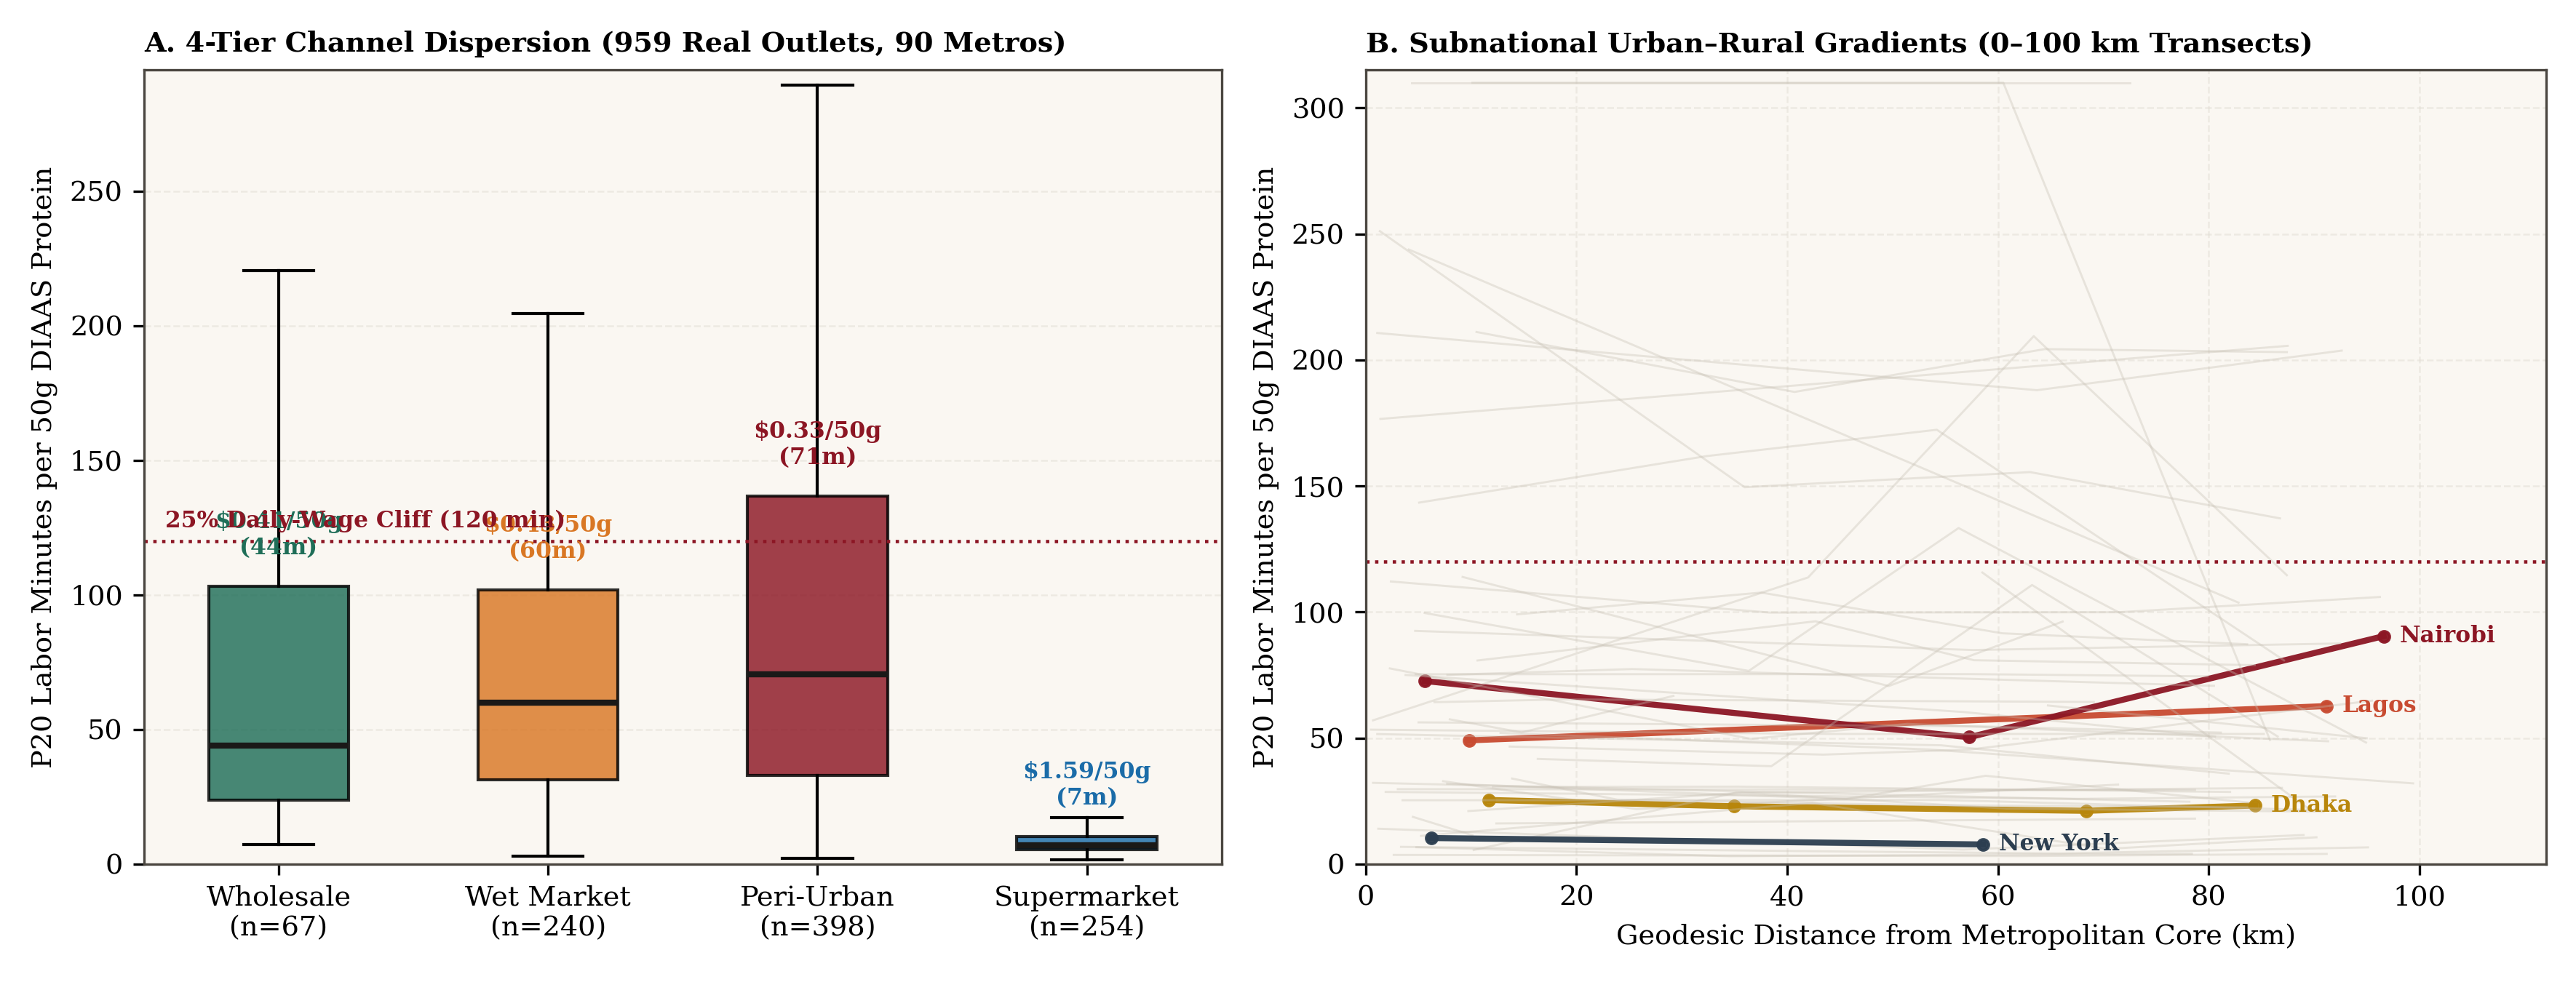
\includegraphics[width=0.96\textwidth]{figures/fig2_complementarity_validation.png}
\caption{\textbf{Spatial generalization and market hub proximity diagnostics.} Contiguous $5^\circ \times 5^\circ$ block cross-validation confirms robust out-of-sample generalization across continents while high hub density anchors $94.4\%$ of the global population within $100\text{ km}$ of direct price observations.}
\label{fig:validation}
\end{figure}

\section{Usage Notes \& Code Availability}

\subsection{Recommended Analytical Practices}
Researchers reusing these data artifacts should observe three methodological conventions:
\begin{itemize}
    \item \textbf{Population Weighting:} When aggregating H3 Resolution-4 cells in \texttt{h3\_weather\_grid.json} to national or regional statistics, weight cell-level metrics (\texttt{u\_usd}, \texttt{w\_med}, \texttt{w\_p20}, \texttt{labor\_min\_med}) by \texttt{pop} rather than computing unweighted cell averages, as cell area varies slightly with latitude and uninhabited cells are excluded.
    \item \textbf{Consumer Whole Foods vs.\ B2B Ingredient Parity:} In \texttt{gvk\_density\_and\_frontiers.json}, the $15$ \texttt{regime\_curves} represent consumer-ready whole foods and retail staples, whereas the $2026$ bioreactor and single-cell markers represent factory-gate B2B protein isolates requiring downstream formulation, lipid/carbohydrate pairing, and retail packaging. Analysts should not compare unformulated B2B isolate costs directly against retail household food baskets without adding retail formulation margins.
    \item \textbf{Uncertainty Propagation:} For econometric regressions using interpolated cells beyond $100\text{ km}$ from an observed market hub (\texttt{dist\_hub\_km > 100}), we recommend clustering standard errors at the $5^\circ \times 5^\circ$ spatial block level or weighting by inverse prediction variance.
\end{itemize}

\subsection{Reproducibility and Verification Script}
All code and processed JSON artifacts are archived under version tag \texttt{v1.0-2026}. Prior to downstream analysis, users can verify bit-for-bit file integrity and biophysical invariants by running:
\begin{verbatim}
python REPLICATION_MANIFEST.py
\end{verbatim}
which audits the SHA-256 cryptographic checksum of each JSON file in \texttt{public/data/} and re-verifies $\text{LP}_{v,i} \ge \text{LP}_i$ across all $70{,}440$ H3 Resolution-4 cells.

\begin{thebibliography}{9}
\bibitem{fao2013}
Food and Agriculture Organization of the United Nations (FAO). \textit{Dietary Protein Quality Evaluation in Human Nutrition: Report of an FAO Expert Consultation}. FAO Food and Nutrition Paper 92 (FAO, Rome, 2013).

\bibitem{fao2024}
FAO, IFAD, UNICEF, WFP \& WHO. \textit{The State of Food Security and Nutrition in the World 2024: Financing to End Hunger, Food Insecurity and Malnutrition in All Its Forms} (FAO, Rome, 2024).

\bibitem{nordhaus1996}
Nordhaus, W. D. Do real-output and real-wage measures capture reality? The history of lighting suggests not. In \textit{The Economics of New Goods} (eds Bresnahan, T. F. \& Gordon, R. J.) 29--66 (University of Chicago Press, 1996).

\bibitem{gabrielli1950}
Gabrielli, G. \& von K\'arm\'an, T. What price speed? Specific power required for propulsion of vehicles. \textit{Mechanical Engineering} \textbf{72}, 775--781 (1950).

\bibitem{allen2001}
Allen, R. C. The great divergence in European wages and prices from the Middle Ages to the First World War. \textit{Explorations in Economic History} \textbf{38}, 411--447 (2001).

\bibitem{roberts2017}
Roberts, D. R. et al. Cross-validation strategies for data with temporal, spatial, hierarchical, or phylogenetic structure. \textit{Ecography} \textbf{40}, 913--929 (2017).

\bibitem{headey2019}
Headey, D. D. \& Alderman, H. H. The relative caloric prices of healthy and unhealthy foods differ systematically across income levels and continents. \textit{The Journal of Nutrition} \textbf{149}, 2020--2033 (2019).

\bibitem{bai2021}
Bai, Y., Alemu, R., Block, S. A., Headey, D. \& Masters, W. A. Cost and affordability of nutritious diets at retail prices: Evidence from 177 countries. \textit{Food Policy} \textbf{99}, 101983 (2021).
\end{thebibliography}

\end{document}
